\begin{artengenv}{Sebastian J. Szybka}
	{Some remarks on the first image of a black hole}
	{Some remarks on the first image of a black hole}
	{Some remarks on the first image of a black hole}
	{Astronomical Observatory, Jagiellonian University\\
	Copernicus Center for Interdisciplinary Studies}
	{On the 10\textsuperscript{th} of April, 2019 the Event Horizon Telescope Collaboration presented the first image of the black hole. The image was obtained with a planet-scale array of eight ground-based radio telescopes. The observation relied on a technique called very long base interferometry which synchronises telescope facilities around the world. The image of a black hole together with the recent detections of gravitational waves confirms one of the most intriguing predictions of Einstein's gravity theory, namely, the existence of black holes. I will provide more details on this remarkable observation and explore its consequences for our understanding of nature. The physical reality of black holes is strongly supported by recent advances of astronomy. I claim that this fact is the key to understanding the relation between our world and the world of mathematics.}
	{black holes, event horizon, general relativity, interferometry, astronomy, Einstein, geometry.}


\section{Introduction}
\indent \lettrine[loversize=0.13,lines=2,lraise=-0.05,nindent=0em,findent=0.2pt]%
{T}{}he mysterious relation between mathematics and physical world was and still is a subject of a debate \parencite{wigner_unreasonable_1960}. From the standpoint of a theoretical physicist, but not a professional philosopher, I must admit that existence of black holes is one of the sharpest proofs of the idea that underlying structure of the physical world is of the mathematical nature. 

Black holes are the essence of general relativity. After one learns general relativity and the mathematics of black holes, one cannot help feeling that one has gained some deep insight into how nature works\footnote{Paraphrasing the words of Robert Wald \parencite*{wald_general_1984}.}.  However, as pointed out by Richard Feynman \parencite*{feynman_character_1967}, this feeling is based on a personal experience and as such is not easy to communicate outside physicist's scientific community because  [without mathematics---author's note] \textit{it is difficult to get across a real feeling as to the beauty, the deepest beauty, of nature}. Although \textit{physicists cannot make a conversion to any other language} [than mathematics---author's note], I believe, that from time to time, all of us are given a chance to appreciate a glimpse of the nature's beauty directly with our senses, just by looking at it. Recently, a glimpse of a charm of black holes was revealed to millions of people around the globe.

The scientific impact of the first image of a black hole may be less profound than the impact of the recent gravitational waves detections, but seeing is believing. The image of the black hole presented to the public by the Event Horizon Telescope Collaboration\footnote{The results were published on the 10\textsuperscript{th} of April in the six papers in a special issue of \textit{The Astrophysical Journal Letters}, \parencite[see e.g.][]{the_event_horizon_telescope_collaboration_first_2019}. More about Event Horizon Telescope Collaboration, \parencite[see][]{noauthor_event_nodate}.} is groundbreaking for the perception of black holes as real objects, especially beyond the scientific community. 

\section{Black holes}

Black holes are fascinating objects because there are made only from our concepts of space and time\footnote{The most important black hole spacetimes are given by the solutions to the vacuum Einstein's equations.}---no matter involved! They are regions of `no return' separated from the remaining part of the Universe by the boundary called an event horizon. Their existence is essential for our understanding of what time and space are. 

The history of black holes is integral to understanding the relation between real world and mathematics \parencite{malec_black_2018}. If we skip Newtonian `dark stars' and move directly to proper Einsteinian black holes, than a remarkable fact must be mentioned. The black hole concept was not invented by anyone. As far as I know, existence of objects made of space and time not only exceed imagination of scientists, but even seemingly unfettered imagination of storytellers. The existence of black holes was dictated to us by the mathematical structure of Einstein's general relativity. In fact, many scientists, including the father of general relativity---Albert Einstein---were very reluctant to accept their physical reality.

Not only origins of black holes were mathematical. As we believe today, the real astrophysical black holes are macroscopic physical objects which have properties that are believed to be typical for mathematical structures (not physical one). The mathematical model of a coffee cup is only an approximation---it is \textit{similar} to the physical coffee cup. The model may be, of course, useful in, e.g., calculating the volume of the coffee cup. Two coffee cups, even if they belong to the same tableware, are never identical, so a single mathematical model cannot be identified with them. Definitely, the mathematical model of the coffee cup is not a coffee cup. In contrast to that, electrons and their mathematical description cannot be easily separated. For example, we have a good reason to believe that the electric charge of one of the electrons in my body and the electric charge of one of the electrons in the distant galaxy billions light years away are exactly the same. Electrons' charges are identical. Two electrons are not like two cups from the same tableware. If we neglect their extrinsic properties, they cannot be distinguished at all.  The property of being \textit{identical}, in contrast to being \textit{similar}, is a mathematical property not a physical one \parencite{staruszkiewicz_filozofia_2001}. Of course, our contemporary mathematical description of the electron is not `an electron.' However, it seems that the mathematical structure which we have discovered seems to approximate the deeper mathematical structures which cannot be separated from the physical objects they define. In electrodynamics, the equality of electric charges of electrons does not follow from any basic principles, but was introduced by physicists to obtain the theory that matches observations. Nevertheless, this property of electrons fits to the physical world so well that is seems indispensable in any future theory of electrons.\footnote{Such strange coincidences are known in the history of physics. In the Newtonian mechanics, gravitational mass and inertial mass of a body are separate concepts. The equality of both masses was an assumption which needed to be confirmed by observations. In contrast to that in the Einstein's theory, gravitational mass and inertial mass correspond to a single concept---they are `the same.'}

For us, the microscopic world of particles is elusive because it is not directly accessible to our senses.  The black holes are macroscopic objects that share with electrons this amazing property of being realisations of a simple mathematical structure. The charges of two electrons are indistinguishable in the same sense as two equal numbers are identical. Whenever a stationary astrophysical black hole has a several solar masses or billions of solar masses it is defined by only two parameters: the mass and angular momentum. This universality extends over ten orders of magnitude. Any two such black holes are identical (if we ignore different values of parameters), in the same sense, as two mathematical functions are. In contrast to electrons, astrophysical black holes are large which makes them, in principle, accessible to our senses. Observations of them reveal directly mathematical nature of reality. As pointed out by the world-famous astrophysicist and Nobel laureate Subrahmanyan Chandrasekhar \parencite*{chandrasekhar_shakespeare_1975}:

\myquote{
In my entire scientific life, extending over forty-five years, the most shattering experience has been the realization that an exact solution of Einstein's equations of general relativity, discovered by the New Zealand mathematician Roy Kerr, provides the absolute exact representation of untold numbers of massive black holes that populate the universe. This ``shuddering before the beautiful'' this incredible fact that a discovery motivated by a search after the beautiful in mathematics should find its exact replica in Nature, persuades me to say that beauty is that to which the human mind responds at its deepest and most profound level.}

There is at least one more important secret hidden inside of black holes. The edge of the Universe is usually related to the so-called particle horizon. This boundary of the observable Universe is really far away. Although we cannot observe what lays behind it, we have some reasons to believe that nothing unusual happens there. The true mysterious edge of spacetime is not there, but, in the cosmological scales, it lays just behind the corner. The Einstein's gravity theory---general relativity---predicts its own breakdown inside of the black holes. This means that space and time, as we know it, ends there. Therefore, the black holes are true gates to the unknown territory that cannot be explored without the new physics.

\section{Casting call}

If we look at a night sky with naked eyes, we see mainly photons emitted by Milky Way stars. However, if we observe a sky with a help of a radio telescope, one of the brightest sources are massive black holes (black holes are black, but the accreting matter radiates energy away). In this sense, we have already indirectly observed black holes for many years. However, by \textit{seeing} one usually means to see a shape of an object. This is not easy task for astronomers. The universe is vast, distances are huge. Modern sky surveys catalogue billions of stars, but, only images of several dozen of them has been resolved. Majority of stars are seen as point sources. 

Taking an image of a black hole is a formidable task. Masses of some galactic black holes may reach dozens of billion of solar masses, but black holes are most compact objects in the Universe. For example, the black hole with the mass equal to the mass of Earth is really tiny---its radius is only about $9$ mm. 

As we known today, astrophysical black holes exist in two sizes. The so-called stellar black holes with masses ranging from several to dozens of solar masses are created as an end state of evolution of massive stars. The so-called galactic black holes (or supermassive black holes) with masses ranging from hundreds of thousands to tens of billions of solar masses reside in the center of galaxies. The black holes are black, so good candidates for taking an image must be active---they must swallow the surrounding matter:  a cosmic dust, a gas, stars. The matter falling on a black hole radiates huge amount of energy which lighten up the neighbourhood and creates the black hole shadow. The black hole shadow contains the event horizon, thus we expected to see a gate to the region of `no return.' The candidates must also have possibly large angular size---this parameter is crucial for resolving images. It turns out that in this competition the supermassive black holes are clear winners. The Event Horizon Telescope team picked out two candidates: the nearest supermassive black hole Sgr A* at the center of our galaxy and much bigger supermassive black hole at the center of the galaxy M87. Our supermassive black gole Sgr A* is about 26000 light years away from Earth and has about four million solar masses. The M87 black hole is about 1500 times more massive and 2000 times further away. It follows from this comparison that the size of the M87 black hole event horizon is only about 22 micro-arc-sec of a degree compared to 53 micro-arc-sec of a degree of Sgr A*. Nevertheless, the M87 black hole turned out to be a better candidate. Although the Event Horizon Telescope team attempted to create images of both black holes only the image of the M87 black hole was presented on the 10\textsuperscript{th} of April 2019. The center of our galaxy is not a best direction to conduct this kind of imaging. The larger mass of the M87 black hole implies that the image change less during observation time which guarantees more stable condition for taking an image. Photographing a running athlete with long exposure time is definitely much harder than taking a photo of grandparents behind a table!

\section{Your camera matters}

How to create an image of a black hole? Since the event horizon of the M87 black hole is about 22 micro-arc-sec of a degree as seen from Earth, an extreme resolution is needed. A resolution of a human eye is about 60 arc-sec of a degree. The Hubble telescope is much better having a resolution about 0.05 arc-sec of a degree, but still nowhere close to what is needed. We need an instrument which would allow a person sitting in Kraków to read a newspaper in New York! A simple rule says: the larger diameter of the lens the higher resolution. The formula which is necessary to estimate the size of the instrument has a trivial form. The resolution of an astronomical instrument is about $\lambda/D$ where $\lambda$ is the wavelength of the electromagnetic radiation at which we want to observe and $D$ is the size of the instrument. Firstly, the Event Horizon Telescope team had to decide at which wavelength they want to observe a black hole. Several factors must be taken into account here: longer wavelengths require bigger instruments, the M87 black hole should look interesting at a given wavelength, wavelengths at which the Earth-based astronomical observations are conducted are strictly restricted by absorption of the Earth's atmosphere. Majority of people would like to have a photograph of a black hole and by that they usually mean: in the visible light. However, the wavelength of the electromagnetic waves is not their fundamental property---it depends on the observer who measures them. There is no fundamental difference between photons associated to the visible light and those associated to radio waves. The techniques used to capture them differs because these photons have different energies relative to us, but what is infrared radiation for one observer may be visible light to another observer who moves relative to the first one at relativistic speed. Therefore, for a professional astronomer the image of the black hole in different part of the electromagnetic spectrum than the visible range is not less `true' nor interesting than a photograph in the visible light. (Even cameras in ordinary mobile phones go slightly beyond visible part of the spectrum.) Moreover, it was expected that our black holes do not look attractive from this distance in the visible light---they would probably look more like an ordinary stars and we would not see a black hole shadow. Observations in standard radio waves were not convenient because necessary resolution would imply too large size of the instruments (from formula $\lambda/D$). It turned out that the wavelength $1.3$ mm is the best choice: it was expected that we will see the black hole shadow, there is the so-called `atmospheric window' at this wavelength (a tiny one), and, what a lucky coincidence, the M87 black hole is just at the right distance, hence, the instrument has the largest admissible size---the size of Earth!

Of course, building an astronomical instruments of the size of Earth is not for faint-hearted. Astronomical instruments used to detect electromagnetic waves at $1.3$ mm do not resemble optical telescopes. They are radio telescopes and have a form of a satellite antenna---a dish. The world-largest radio dish telescope FAST has a $500$ m aperture (and a fixed dish). Several years ago building a radio telescope of the size of Earth would not be possible at all. However, recently, the technique called the very long base line interferometry (VLBI) has been developed and successfully applied in astronomical observations. 

Imagine that the dish of our satellite antenna has a hole. It will still work, but less efficiently. The size of the astronomical instrument $D$ that enters the formula for a resolution $\lambda/D$ denotes the distance between most distant parts of our instrument. Therefore, a dish with many holes would have the same resolution as the dish without holes, but the signal would be much weaker. The basic idea of the VLBI technique is to use many different instruments spread across the globe and integrate the signal. Thus, all of them may work as a single instrument. The clear advantage of this method is that there is no need to build a new instrument and one may use pre-existing infrastructure. The basics of this technique has been established many years ago, but only recently the technical difficulties were overcome. The highly non-trivial task is to correlate the signal between different instruments. One should know with extremely high precision when the signal arrived. Clocks at different observatories must be precise and synchronized. A delay of the signal that is usually induced by the telescope electronics, must be estimated to high accuracy. All these goals were achieved by the Event Horizon Telescope team. The atomic clocks used to time-stamp data were hydrogen masers. These clocks lose only one second in every 100 million years. The required synchronisation obtained with the Global Positioning System was at the level of a millionth of a second.

The signal from the black hole which the Event Horizon Telescope Collaboration was going to observe was weak. In fact, it was billion times weaker than the electromagnetic signal received by an old-fashion TV antenna. Nevertheless, the array of eight radio telescopes (ALMA, APEX, the IRAM 30-meter telescope, the James Clerk Maxwell Telescope, the Large Millimeter Telescope Alfonso Serrano, the Submillimeter Array, the Submillimeter Telescope, and the South Pole Telescope) was powerful enough to observe the M87 black hole during a week long session. (The Event Horizon Telescope project has been in the works for two decades to make this observations possible.) The radio telescopes do not create images as `single shots.' They rather work like scanners which measure intensity of the radiation at a given point. The instruments recorded hundreds of petabytes of data which was combined into a single image by supercomputers at the Max Planck Institute for Radio Astronomy and MIT Haystack Observatory. (What is interesting, it was faster to transport hard disks with data on planes than send data in a digital form over internet.) 

\section{Seeing is believing}

The image of the black hole at the center of the galaxy M87 is presented in figure \ref{bh}. The black hole was observed at a single wavelength $1.3$ mm, thus the gradation in color\edtfootnote{The printed format of this article contains black-and-white graphics, the electronic format is prepared in color.} does not corresponds to different wavelengths, but to the brightness (colors are artificial). The matter falling onto black hole forms an accretion disk. It is heated and glows. The gravity bends light which forms a bright ring around a dark shadow of the black hole. For a non-spinning black hole (but this black hole is spinning) the inner radius of the ring is about $2.6$ times bigger then the radius of the event horizon. At first sight, it looks like we see the M87 black hole in the direction perpendicular to the disk. This is not true. The light rays are bend so strongly that we see also the part of the accretion disk which should be hidden behind the black hole. One part of the ring is brighter, because of the so-called relativistic beaming effect: the increased brightness implies that this part of the accretion disk rotates towards us.
%
\begin{figure}[t!]
\begin{center}
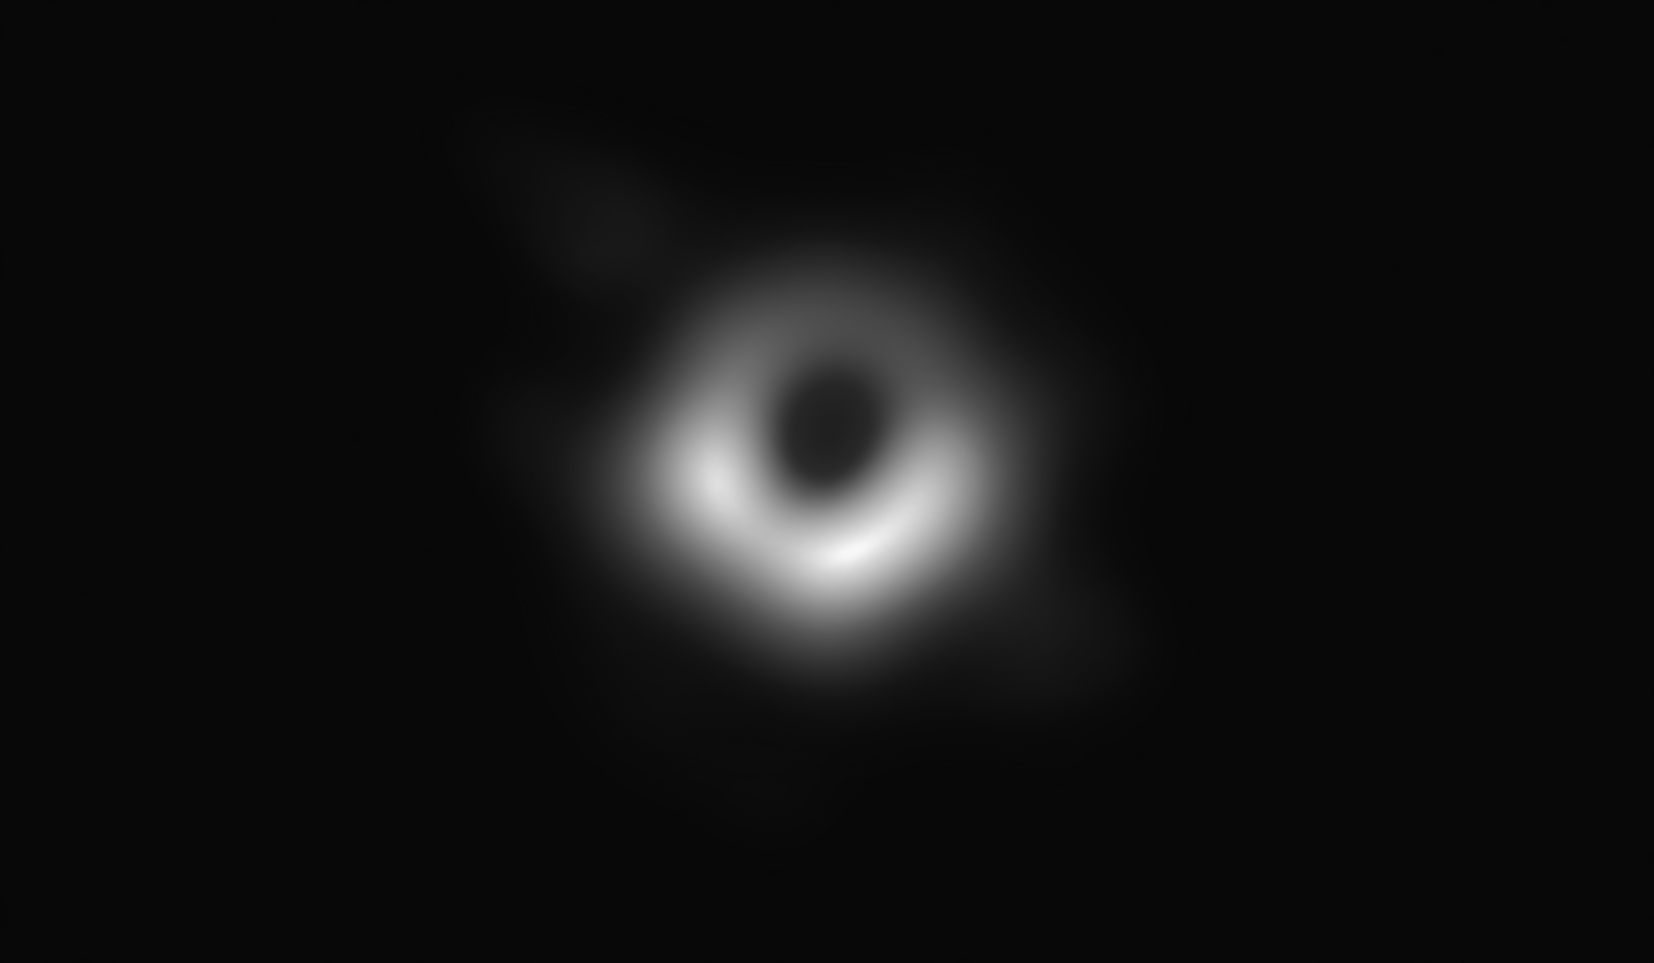
\includegraphics[width=\textwidth]{ART_Szybka/szybka-imgbw.png}
%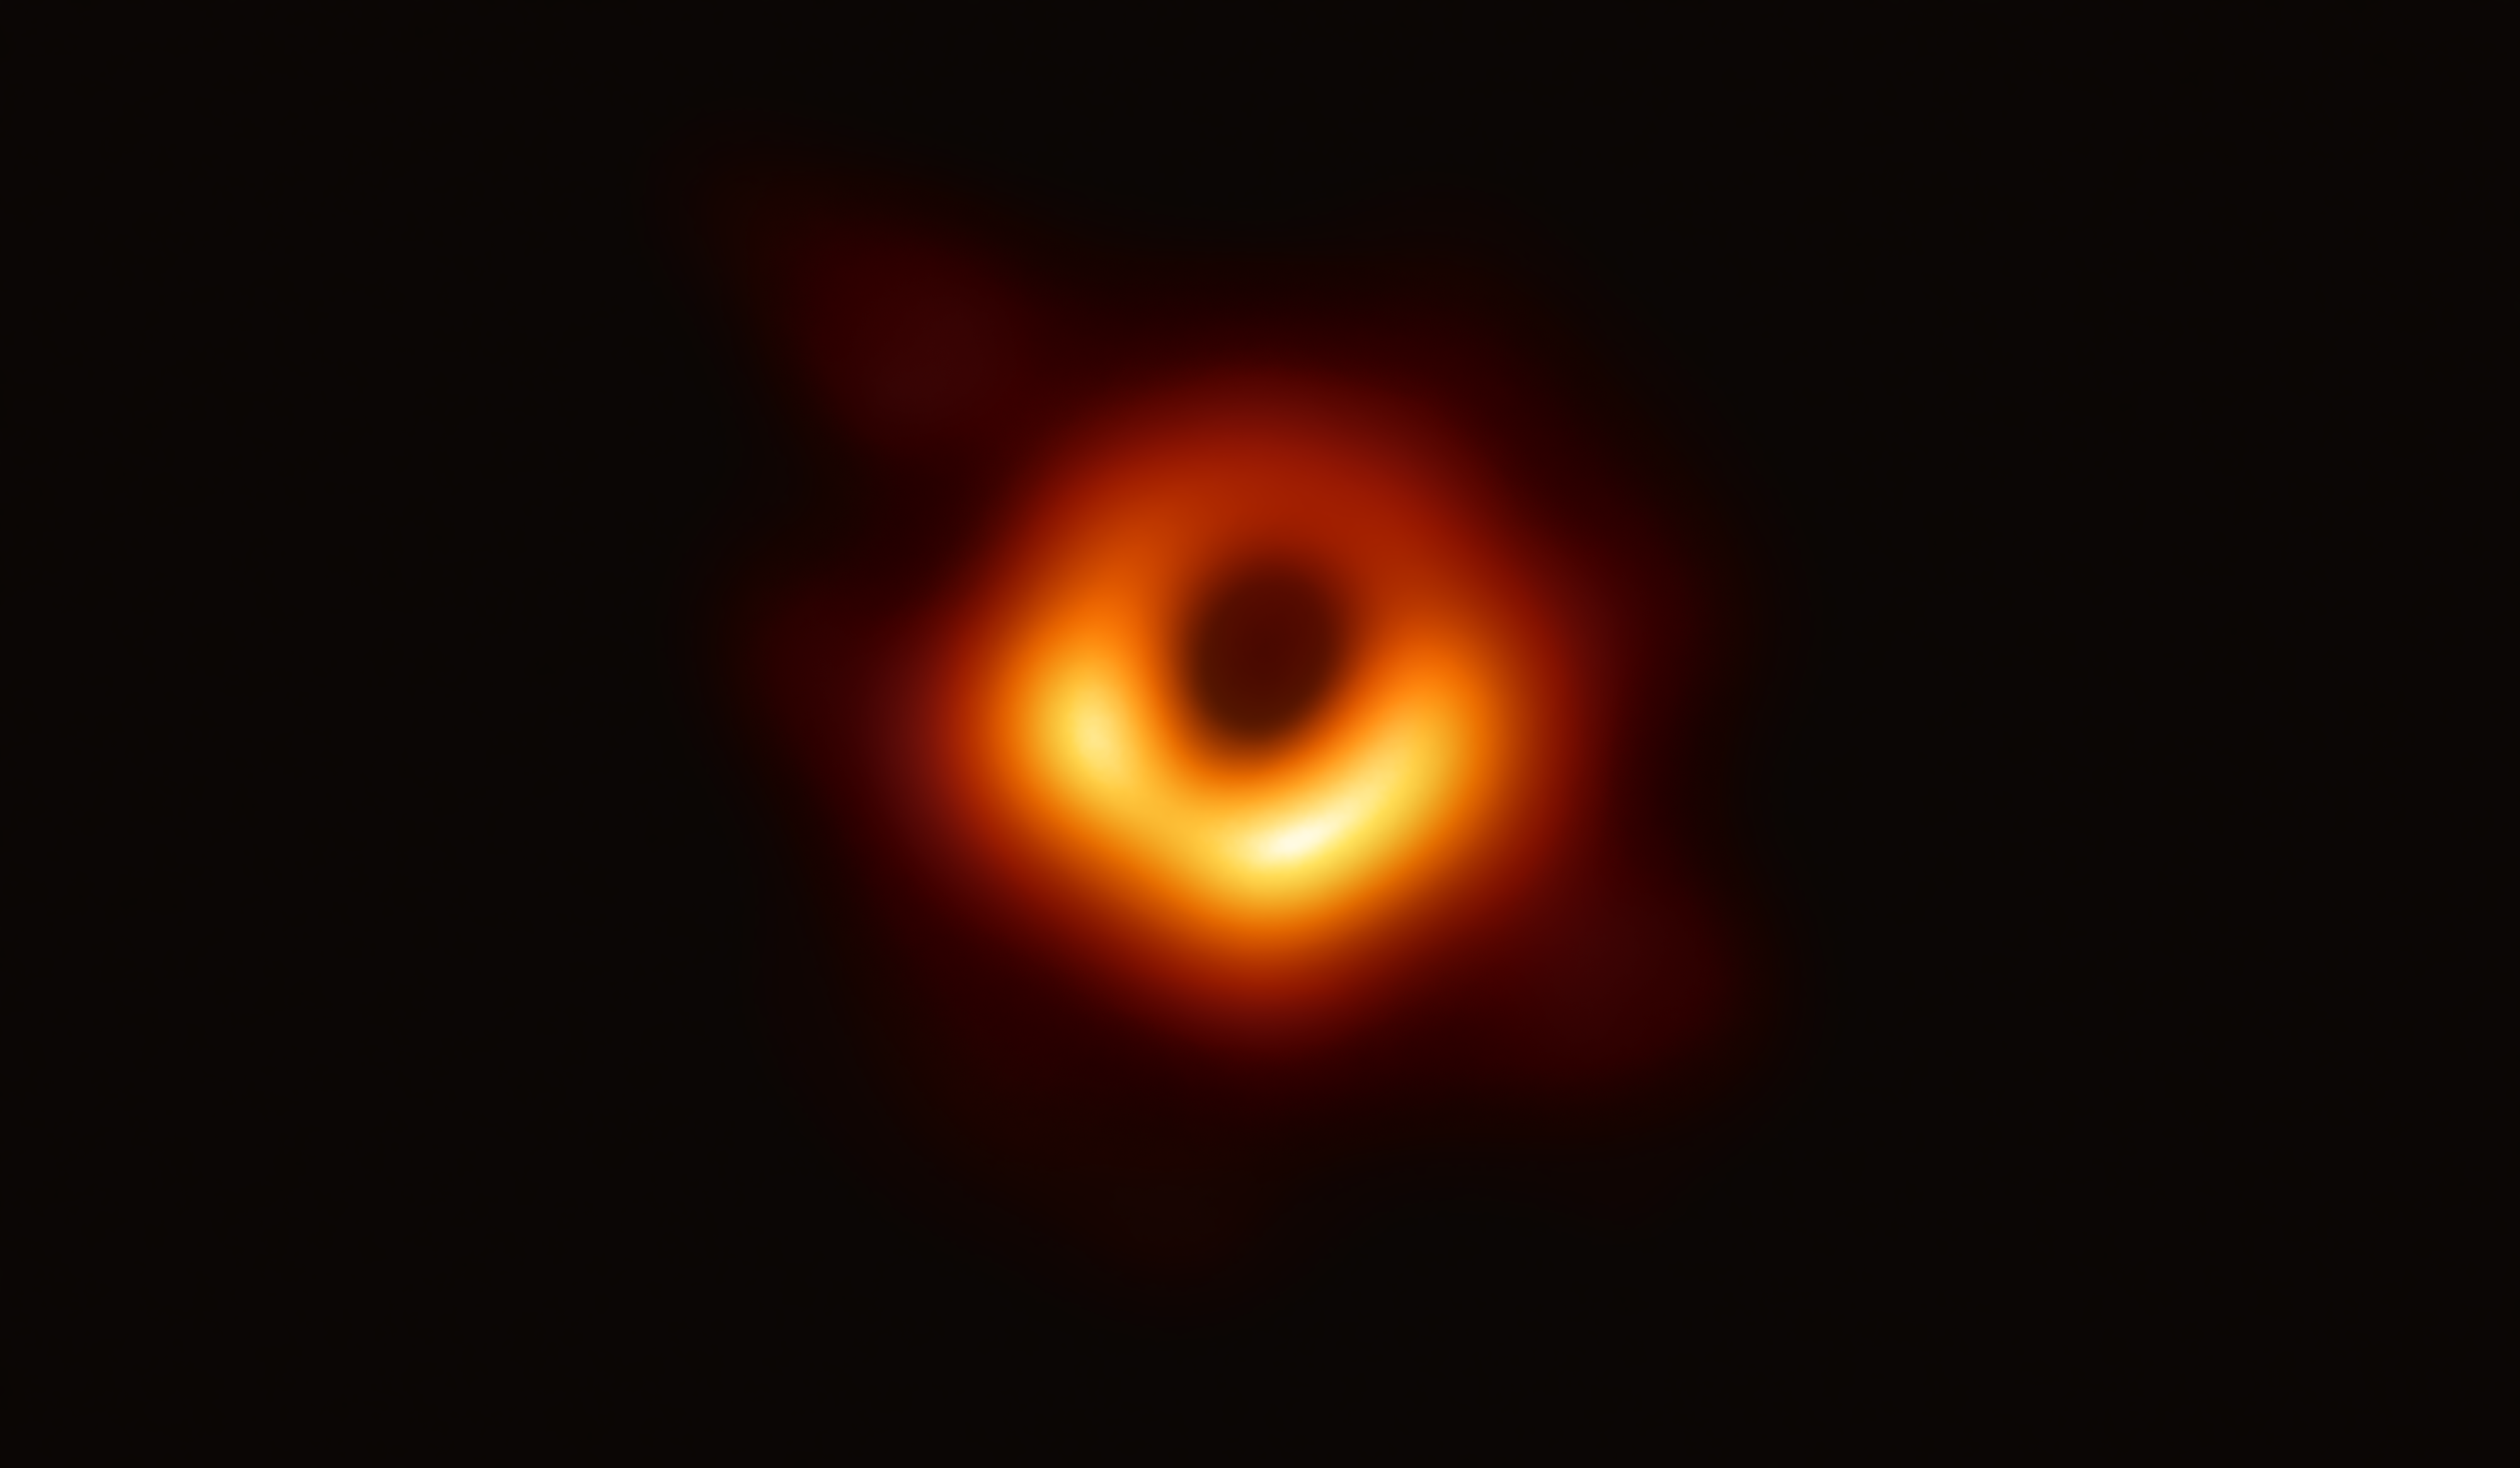
\includegraphics[width=\textwidth]{ART_Szybka/szybka-img.png}
\caption{The image of the supermassive black hole at the center of the galaxy M87 (the black hole is $6.5$ billion times more massive than the Sun). The matter falling on the black hole shines radiating energy away. The extreme gravity curves light which forms a bright ring in the image. At the center of the ring a dark silhouette of the black hole is clearly visible. This shadow contains the event horizon. Credit: Event Horizon Telescope Collaboration.}
\label{bh}
\end{center}
\end{figure}
%

 The M87 black hole is 55 million light year from Earth and is 6.5 million times more massive than the Sun. Its event horizon radius is about $120$ times larger than the distance from Earth to the Sun (three times larger than the average distance between Pluto and the Sun).

The first image of the black hole (figure \ref{bh}) is consistent with general relativity. Of course, there are many other images that would be consistent with the Einstein's gravity theory (depending on the parameters of the system), thus in this case it is better to talk about consistency than a direct proof of the theory. Nevertheless, many characteristic features of this image agree with predictions of general relativity and one may use it to improve estimates of the M87 black hole parameters (like a mass and a size). With a help of this image we may exclude some exotic alternatives to black holes. 

\section{Summary}

The image obtained by the Event Horizon Telescope Collaboration (with 200 scientist involved) was a spectacular example of application of very large base interferometry. The breakthrough in technology and new algorithms allowed the team to achieve something that not so long time ago was presumed to be impossible. What is even more important: the future is bright. The first image of the black hole which was presented on the 10\textsuperscript{th} of April 2019 was not a final product of the project, but just a first outcome. With more instruments joining the Event Horizon Telescope Collaboration and increased sensitivity we should expect more spectacular images of the M87 black hole and other black holes. Probably, in not so distant future, we may even expect  movies showing the black holes in action. 

The recent detections of gravitational waves from colliding black holes and the image of the black hole are remarkable achievemnts. Any doubts about the reality of black holes slowly dissolve. Their existence must be taken seriously. In my opinion, this fact sheds light on fundamental philosophical questions such as relation between the real world and mathematics. We may directly observe macroscopic physical entities which are inseparable from their mathematical description. 

For those, who have seen \textit{La Porte de l'Enfer} by August Rodin, the image of the M87 black hole may have a special poetic meaning. Look again at figure \ref{bh}. There is the event horizon at the central part of the black hole silhouette. Not far behind it a singularity is hidden. The space and time as described by modern physics ceases to exist there. Behind the curtain of the event horizon the known ends and unknown begins, the flow of time twirls. The laws of physics tells us: abandon all hope for the return, who enters here.

\end{artengenv}